\documentclass[12pt,answers]{exam}
\usepackage{fontspec,graphicx,circuitikz,amsmath}
\setmainfont{Times New Roman}

\headheight 8pt \headsep 20pt \footskip 30pt
\textheight 9in \textwidth 6.5in
\oddsidemargin 0in \evensidemargin 0in
\topmargin -.35in

\begin{document}
\begin{center}
\LARGE CSE435 Introduction to EDA \& Testing - Spring 2022 \\
\Large Homework Assignment \#1 \\
\Large Shao-Hsuan Chu - B073040018 \\
\end{center}
\bigskip

\begin{questions}
  \question (25\%) If the yield of good dice is 90\%, and we want a defect level not to exceed 0.1\%, what level of testing in terms of fault coverage must be achieved?
  \begin{solution}
  The defect level $\textbf{DL}$ can be obtained by $\textbf{DL} = 1 - \textbf{Y} ^ {1 - \textbf{T}}$, where $\textbf{Y}$ is the yield, indicating the manufacturing capability, and $\textbf{T}$ is the fault coverage, indicating the testing capability.
\begin{align*} 
0.001                             &\geq 1 - 0.9 ^ {1 - \textbf{T}} \\
0.9 ^ {1 - \textbf{T}}            &\geq 1 - 0.001 \\
0.9 ^ {1 - \textbf{T}}            &\geq 0.999 \\
\log_{0.9} 0.9 ^ {1 - \textbf{T}} &\leq \log_{0.9} 0.999 \\
1 - \textbf{T}                    &\leq 0.0095 \\
\textbf{T}                        &\geq 0.9905 = 99.05\%
\end{align*}
\textbf{Answer:} The fault coverage $\textbf{Y}$ must be at least 99.05\%

  \end{solution}

  \question (50\%) Given the market entry time verse revenue curves as shown in Figure 1, fill in the following formula
  \begin{center}
  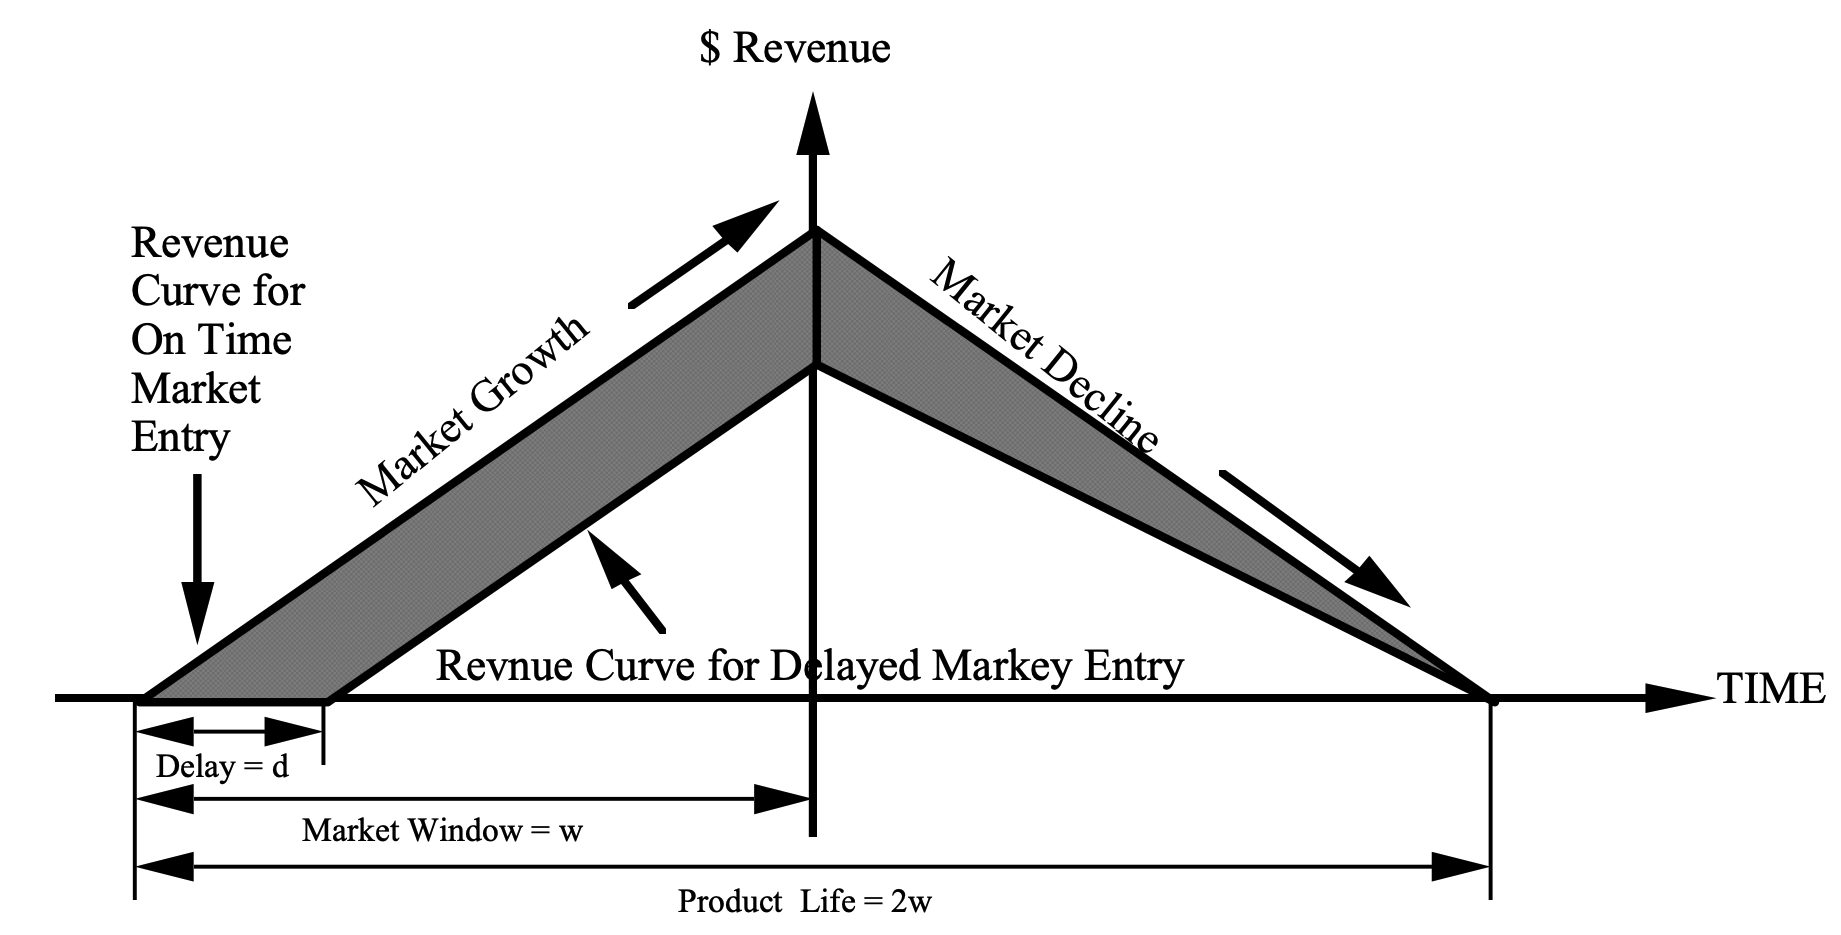
\includegraphics[width=0.8\textwidth]{assets/q2.png}
  \end{center}
  \begin{parts}
    \part (25\%) Lost Revenue = Total Expected Revenue * [\quad ]. The answer should be in term of $d$ and $w$. $d$ is the delay entry, $2w$ is the product life. The two market growth rates are the same.
    \begin{solution}
    The Lost Revenue $\textbf{LR}$ equals to the absolute difference between the Total Expected Revenue $\textbf{TER}$ and the Total Actual Revenue $\textbf{TAR}$. Denote the market growth rates as $r$, the Lost Revenue can be obtained by
\begin{align*}
\textbf{TER} &= \frac{1}{2} (2w) (w)r = (w^2) r \\
\textbf{TAR} &= \frac{1}{2} (2w - d) (w-d)r = (w^2 - \frac{3}{2}wd + \frac{1}{2}d^2) r \\
\textbf{LR}  &= \textbf{TER} - \textbf{TAR} \\
\textbf{LR}  &= (\frac{3}{2}wd - \frac{1}{2}d^2) r \\
\textbf{LR}  &= \textbf{TER} \times \frac{(\frac{3}{2}wd - \frac{1}{2}d^2) r}{\textbf{TER}} \\
\textbf{LR}  &= \textbf{TER} \times \frac{\frac{3}{2}wd - \frac{1}{2}d^2}{w^2} \\
\end{align*}
\textbf{Answer:} $(\frac{3}{2}wd - \frac{1}{2}d^2) / w^2$

    \end{solution}

    \part (25\%) Given a product with total expected revenue \$100M, product life is 20 months. What is the revenue loss due to the one month late to the market?
    \begin{solution}
    
\begin{tabular}{rlcc|c|c|c|c|c|c|}
  \specialrule{.1em}{.05em}{.05em} 
  \multirow{2}{*}{Step} &
  \multirow{2}{*}{Comments} &
  \multicolumn{7}{c}{Cube} \\
  \cline{3-10}
  && \multicolumn{1}{|c|}{a} & b & c & d & e & f & g & h \\
  \specialrule{.1em}{.05em}{.05em} 
  1 &
  Activate f-sa1. TC(0) = PDCF &
% \multicolumn{1}{|c|}{a} & b & c & d & e & f & g & h \\
  \multicolumn{1}{|c|}{ } &   & 1 &   & 1 & D'&   &   \\
  \hline
  2 &
  Backward implication: SC\textsubscript{G1} &
% \multicolumn{1}{|c|}{a} & b & c & d & e & f & g & h \\
  \multicolumn{1}{|c|}{\textbf{0}} & \textbf{0} &   &   & 1 &  &   &   \\
  & TC(1) = TC(0) $\cap$ SC\textsubscript{G1} &
% \multicolumn{1}{|c|}{a} & b & c & d & e & f & g & h \\
  \multicolumn{1}{|c|}{0} & 0 & 1 &   & 1 & D'&   &   \\
  \hline
  3 &
  Propagate fault. D-drive = G4. PDC\textsubscript{G4} &
% \multicolumn{1}{|c|}{a} & b & c & d & e & f & g & h \\
  \multicolumn{1}{|c|}{ } &   &   &   &   & D'& 0 & D \\
  & TC(2) = TC(1) $\cap$ PDC\textsubscript{G4} &
% \multicolumn{1}{|c|}{a} & b & c & d & e & f & g & h \\
  \multicolumn{1}{|c|}{0} & 0 & 1 &   & 1 & D'& 0 & D \\
  \hline
  4 &
  Backward implication: SC\textsubscript{G3} &
% \multicolumn{1}{|c|}{a} & b & c & d & e & f & g & h \\
  \multicolumn{1}{|c|}{ } &   & 1 & \textbf{0} &   &   & 0 &   \\
  & TC(3) = TC(2) $\cap$ SC\textsubscript{G3} &
% \multicolumn{1}{|c|}{a} & b & c & d & e & f & g & h \\
  \multicolumn{1}{|c|}{0} & 0 & 1 & 0 & 1 & D'& 0 & D \\
  \hline
  5 &
  \multicolumn{9}{l}{No justification needed. Test generated.} \\
  \specialrule{.1em}{.05em}{.05em} 
\end{tabular}

\textbf{Answer:} (a, b, c, d) = (0, 0, 1, 0).


    \end{solution}
  \end{parts}

  \question (25\%) Try to derive the test pattern for the fault $f$ (sa1). Explain your result. Try to simplify the circuit.

    The test pattern can be given as the table below. Each row is a clock tick, and at the initial tick, $\text{Q}_\text{n}$ is in the don't-care condition. For all the following ticks, $\text{Q}_\text{n}$ is the $\text{Q}_\text{n+1}$ from the previous tick.
\begin{center}
  \begin{tabular}{c c | c | c}
    J & K & $\text{Q}_\text{n+1}$ & Functions \\
    \hline
    0 & 1 & 0 & set 0 \\
    0 & 0 & 0 & hold 0 \\
    1 & 0 & 1 & set 1 \\
    0 & 0 & 1 & hold 1 \\
    1 & 1 & 0 & toggle to 0 \\
    1 & 1 & 1 & toggle to 1 \\
  \end{tabular}
\end{center}
If output does not meet the expectation, a functional fault is detected in the F/F. One of the set, hold or toggle to 0/1 functions could not behave properly.

    \begin{solution}
    The test pattern can be given as the table below. Each row is a clock tick, and at the initial tick, $\text{Q}_\text{n}$ is in the don't-care condition. For all the following ticks, $\text{Q}_\text{n}$ is the $\text{Q}_\text{n+1}$ from the previous tick.
\begin{center}
  \begin{tabular}{c c | c | c}
    J & K & $\text{Q}_\text{n+1}$ & Functions \\
    \hline
    0 & 1 & 0 & set 0 \\
    0 & 0 & 0 & hold 0 \\
    1 & 0 & 1 & set 1 \\
    0 & 0 & 1 & hold 1 \\
    1 & 1 & 0 & toggle to 0 \\
    1 & 1 & 1 & toggle to 1 \\
  \end{tabular}
\end{center}
If output does not meet the expectation, a functional fault is detected in the F/F. One of the set, hold or toggle to 0/1 functions could not behave properly.

    Simplified circuit with stuck-at-1 fault:
\begin{center}
\begin{circuitikz}[line width=.8pt]
  \draw

  %%%%% nand 1

  (0,0)
  node[label=left: $A$] {}
  --
  (3,0)
  node[nand port, anchor=in 1] (nand1) {}

  (0,52 |- nand1.in 2)
  node[label=left: $B$] {}
  --
  (nand1.in 2)

  %%%%% nand 2

  (1.5,-1.5)
  node[not port, anchor=out, scale=0.4] (not1) {}
  --
  (3,-1.5)
  node[nand port, anchor=in 1] (nand2) {}

  (not1.in)
  to[short, -*]
  ++(0, 1.5)

  (0,52 |- nand2.in 2)
  node[label=left: $C$] {}
  --
  (nand2.in 2)

  %%%%% nand 4

  (nand2.out)
  --
  ++(1,0)
  node[nand port, anchor=in 2, number inputs=3] (nand4) {}

  (nand1.out)
  |-
  (nand4.in 1)

  (5,52 |- nand4.in 3)
  node[label=left: $1$] {}
  --
  (nand4.in 3)

  %%%%% F

  (nand4.out)
  --
  ++(0.5,0)
  node[label=right: $F$] {}
  ;
\end{circuitikz}
\end{center}

    \end{solution}
\end{questions}
\end{document}

